% ===== CHAPTER 10 =====
\chapter{电子自旋和自旋-统计定理}
\label{chap:10}
\section{电子自旋}
\label{sec:10.1 Electron Spin}

    所有化学家都熟悉钠原子在火焰中呈现的黄色。事实上,钠原子光谱中最强的黄色线(D线)是两条间隔很近的线。钠的D谱线由激发态$1s^22s^22p^63p$到基态的跃迁产生。\ce{Na} 光谱中这条线和其他线的双线性质表明,价电子可用的预期状态数增加了一倍。

    为了解释原子光谱的这种微观结构,Uhlenbeck 和 Goudsmit 于 1925 年提出,除了电子围绕原子核运动所产生的轨道角动量之外,电子还具有一种\textit{内禀}(内在)角动量。如果我们把电子想象成一个围绕其直径之一旋转的电荷球,我们就能明白这种内禀角动量是如何产生的。因此,我们得到了术语\textbf{自旋角动量}(spin angular momentum),或更简单地,\textbf{自旋}(spin)。然而,电子 “自旋”并不是一种经典效应,电子绕轴旋转的图景并不符合物理现实。内禀角动量是真实存在的,但没有一个容易又直观的模型能够正确解释它的起源。我们不能指望根据宏观世界的经验来理解微观粒子。除了电子,其他基本粒子也有自旋角动量。

    1928 年,狄拉克提出了电子相对论量子力学,在他的研究中,电子自旋自然而然地产生了。

    在我们所局限的非相对论量子力学中,电子自旋必须作为附加假设引入。我们已经了解到,在量子力学中,每种物理属性都有其对应的线性厄米算符。对于轨道角动量等性质,我们可以用相应的算符代替 $p_x$、$p_y$和$p_z$,从经典表达式中构造出量子力学算符。微观粒子固有的自旋角动量在经典力学中没有类似的表达式,因此我们不能用这种方法来构造自旋的算符。为了我们的目的,我们将只使用符号来表示自旋算符,而不给出它们的明确形式。

    与轨道角动量算符$\hat{L}^2, \hat{L}_x, \hat{L}_y, \hat{L}_z$类似,自旋算符也有对应的形式$\hat{S}^2, \hat{S}_x, \hat{S}_y, \hat{S}_z$,假设它们是线性厄米算符。$\hat{S}^2$ 是粒子总自旋角动量大小平方的算符。$\hat{S}_z$ 是自旋角动量在 $z$ 方向上的分量算符。我们有
    \begin{equation}
        \hat{S}^2 = \hat{S}_x^2 + \hat{S}_y^2 + \hat{S}_z^2.
        \label{eq:10.1}
    \end{equation}
    假设自旋角动量算符遵循轨道角动量算符相同的对易关系。与$\left[\hat{L}_x, \hat{L}_y\right] = \mathrm{i} \hbar \hat{L}_z$,$\left[\hat{L}_y, \hat{L}_z\right] = \mathrm{i} \hbar \hat{L}_x$,$\left[\hat{L}_z, \hat{L}_x\right] = \mathrm{i} \hbar \hat{L}_y$[式(\ref{eq:5.46})和(\ref{eq:5.48})],我们有
    \begin{equation}
        \left[\hat{S}_x, \hat{S}_y\right] = \mathrm{i} \hbar \hat{S}_z, \quad
        \left[\hat{S}_y, \hat{S}_z\right] = \mathrm{i} \hbar \hat{S}_x, \quad
        \left[\hat{S}_z, \hat{S}_x\right] = \mathrm{i} \hbar \hat{S}_y.
        \label{eq:10.2}
    \end{equation}
    根据(\ref{eq:10.1})和(\ref{eq:10.2}),通过求得(\ref{eq:5.49})和(\ref{eq:5.50})时所用的算符代数,可以得出
    \begin{equation}
        \left[\hat{S}^2, \hat{S}_x\right] = \left[\hat{S}^2, \hat{S}_y\right] = \left[\hat{S}^2, \hat{S}_z\right] = 0
        \label{eq:10.3}
    \end{equation}
    由于公式 (\ref{eq:10.1}) 和 (\ref{eq:10.2}) 是公式 (\ref{eq:5.107}) 和 (\ref{eq:5.108}) 的形式,根据第 \ref{sec:5.4 The Ladder-Operator Method for Angular Momentum} 节的工作(只取决于对易关系,而不取决于算符的具体形式),可以得出 $\hat{S}^2$ 的本征值为[式(\ref{eq:5.142})]
    \begin{equation}
        \boxed{
            s\left(s+1\right)\hbar^2, \quad s = 0, \frac{1}{2}, 1, \frac{3}{2}, \ldots
        }
        \label{eq:10.4}
    \end{equation}
    以及$\hat{S}_z$ 的本征值为[式(\ref{eq:5.141})]
    \begin{equation}
        \boxed{
            m_s\hbar, \quad m_s = -s, -s+1, \ldots, s-1, s
        }
        \label{eq:10.5}
    \end{equation}

    量子数$s$称为粒子的\textbf{自旋量子数}(spin quantum number)。尽管第 \ref{sec:5.4 The Ladder-Operator Method for Angular Momentum} 节中并没有限制电子的 $s$ 值只能是单一的,但实验表明,所有电子的 $s$ 值都是单一的,即$s = \frac{1}{2}$。质子和中子同样有$s = \frac{1}{2}$。离子有$s = 0$。光子则有$s=1$。然而,公式 (\ref{eq:10.5}) 对光子并不成立。光子在真空中以 $c$ 的速度传播。由于其相对论性质,光子可以有以下两种情况:$m_s = +1$ 或 $m_s = -1$,但不具有$m_s = 0$(见\textit{Merzbacher}, Chapter 22)。这两个 $m_s$ 值分别对应左旋圆偏振光和右旋圆偏振光。

    有了$s = \frac{1}{2}$,电子总自旋角动量的值由(\ref{eq:10.4})的平方根给出:
    \begin{equation}
        \left[\frac{1}{2}\left(\frac{3}{2}\right)\hbar^2\right]^{1/2}=\frac{1}{2}\sqrt{3}\hbar
        \label{eq:10.6}
    \end{equation}
    对于$s = \frac{1}{2}$,式(\ref{eq:10.5})给出了电子$\hat{S}_z$的可能本征值为$+ \frac{1}{2}\hbar$和$-\frac{1}{2}\hbar$。因对应于这些$\hat{S}_z$本征值的电子自旋本征函数由$\alpha$和$\beta$给出:
    \begin{equation}
        \boxed{
            \hat{S}_z \alpha = + \frac{1}{2}\hbar \alpha
        }
        \label{eq:10.7}
    \end{equation}
    \begin{equation}
        \boxed{
            \hat{S}_z \beta = - \frac{1}{2}\hbar \beta
        }
        \label{eq:10.8}
    \end{equation}
    由于$\hat{S}_z$和$\hat{S}^2$可对易,我们可以将$\hat{S}_z$的本征函数变为$\hat{S}^2$的本征函数,有了$s = \frac{1}{2}$和(\ref{eq:10.4})给出的本征值,我们有
    \begin{equation}
        \hat{S}^2 \alpha = \frac{3}{4}\hbar^2 \alpha, \quad
        \hat{S}^2 \beta = \frac{3}{4}\hbar^2 \beta
        \label{eq:10.9}
    \end{equation}
    $\hat{S}_z$和$\hat{S}_x$、$\hat{S}_y$不可对易,所以$\alpha$和$\beta$不是$\hat{S}_x$和$\hat{S}_y$的本征函数。术语\textit{自旋向上}(spin up)和\textit{自旋向下}(spin down)分别指的是$m_s = +\frac{1}{2}$和$m_s = -\frac{1}{2}$。见图10.1。稍后我们将证明,量子数 $m_s$ 的两种可能性会使碱金属光谱中的谱线条数加倍。
    \begin{figure}[ht]
        \centering
        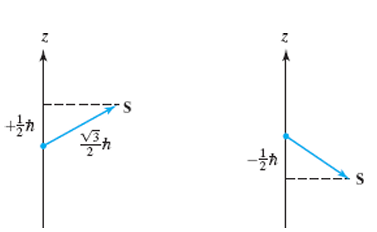
\includegraphics[width=0.4\textwidth]{Figures/10.1.png}
        \caption{
            \centering
            \parbox{\linewidth}{
                \centering 
                电子自旋矢量相对于 $z$ 轴的可能方向。在每种\\
                情况下,$\mathbf{S}$ 都位于以 $z$ 轴为轴的圆锥表面上。
            }
        }
        \label{fig:10.1}
    \end{figure}

    我们之前讨论过的波函数是粒子空间坐标的函数:$\psi = \psi\left(x,y,z\right)$。我们可能想问:自旋本征函数$\alpha$和$\beta$的变量是什么呢?有时,人们在谈论自旋坐标 $\omega$ 时,并没有明确说明这个坐标是什么。通常情况下,人们把自旋量子数 $m_s$ 作为自旋特征函数所依赖的变量。与空间波函数相比,这种程序很不寻常;但因为我们只有两种可能的电子自旋特征函数和本征值,所以这是一种方便的选择。我们有
    \begin{equation}
        \alpha = \alpha\left(m_s\right), \quad
        \beta = \beta\left(m_s\right)
        \label{eq:10.10}
    \end{equation}

    像往常一样,我们希望对本征函数进行归一化处理。单粒子空间波函数的三个变量范围在$-\infty$到$+\infty$之间连续变化,则归一化条件意味着
    \begin{equation*}
        \int_{-\infty}^{\infty} \int_{-\infty}^{\infty} \int_{-\infty}^{\infty} \left|\psi\left(x, y, z\right)\right|^2\: \mathrm{d}x\: \mathrm{d}y\: \mathrm{d}z = 1
    \end{equation*}
    电子自旋本征函数的变量 $m_s$ 只有 $+\frac{1}{2}$ 和 $-\frac{1}{2}$ 两个离散值。因此,对单粒子自旋本征函数的归一化意味着
    \begin{equation}
        \sum_{m_{s}=-1/2}^{1/2} \left|\alpha \left(m_{s}\right)\right|^{2} = 1, \quad \sum_{m_{s}=-1/2}^{1/2} \left|\beta \left(m_{s}\right)\right|^{2} = 1
        \label{eq:10.11}
    \end{equation}
    因为本征函数$\alpha$和$\beta$对应于厄米算符$\hat{S}_z$的不同本征值,所以它们是正交的:
    \begin{equation}
        \sum_{m_{s}=-1/2}^{1/2} \alpha^ * \left(m_{s}\right) \beta \left(m_{s}\right) = 0
        \label{eq:10.12}
    \end{equation}
    令$\alpha\left(m_s\right) = \delta_{m_s, 1/2}$,$\beta\left(m_s\right) = \delta_{m_s, -1/2}$,其中$\delta_{jk}$是Kronecker $\delta$函数,我们就满足了(\ref{eq:10.11})和(\ref{eq:10.12})。

    当我们考虑电子的完全波函数(包括空间和自旋变量)时,我们将根据以下公式对其进行归一化处理
    \begin{equation}
        \boxed{
            \sum_{m_s=-1/2}^{1/2} \int_{-\infty}^{\infty} \int_{-\infty}^{\infty} \int_{-\infty}^{\infty} \left|\psi\left(x, y, z, m_s\right)\right|^2 \:\mathrm{d}x \:\mathrm{d}y \:\mathrm{d}z = 1
        }
        \label{eq:10.13}
    \end{equation}
    符号
    \begin{equation*}
        \int \left|\psi\left(x, y, z, m_s\right)\right|^2 \:\mathrm{d}\tau
    \end{equation*}
    表示对自旋变量求和,对空间变量全范围积分,如 (\ref{eq:10.13}) 所示。符号 $\int \:\mathrm{d}v$ 表示对系统空间变量全范围的积分。

    \begin{quote}
        \small
        \noindent
        电子目前被认为是一种没有子结构的点状基本粒子。高能电子-正电子碰撞实验表明,没有证据表明电子的大小不为零,并将电子半径的上限为$3 \times 10^{-19} \:\mathrm{m}$[D. Bourilkov, \textit{Phys. Rev. D}, \textbf{62}, 076005 (2020); \url{arxiv.org/abs/hep-ph/0002172}.]。质子和中子是由夸克构成的,因此不是基本粒子。质子的均方根电荷半径为$0.88 \times 10^{-15} \:\mathrm{m}$。
    \end{quote}

\section{自旋和氢原子}
\label{sec:10.2 Spin and the Hydrogen Atom}

    具体说明电子状态的波函数不仅取决于$x$、$y$和$z$坐标,还取决于电子的自旋状态。这对氢原子的波函数和能级有什么影响?

    在很好的近似条件下,电子系统的哈密顿算符不涉及自旋变量,而只是空间坐标和关于空间坐标的导数的函数。因此,我们可以将单个电子的定态波函数分离为空间和自旋部分的乘积:
    \begin{equation*}
        \psi\left(x,y,z\right)g\left(m_s\right)
    \end{equation*}
    其中的$g\left(m_s\right)$是$\alpha$或$\beta$的其中之一,取决于$m_s = +\frac{1}{2}$或$m_s = -\frac{1}{2}$。[更一般地,$g\left(m_s\right)$可以是$\alpha$和$\beta$的线性组合;$g\left(m_s\right) = c_1 \alpha + c_2\beta$。]由于哈密顿算符对自旋波函数没有作用,我们有
    \begin{equation*}
        \hat{H} \left[\psi\left(x, y, z\right) g\left(m_s\right)\right] = g\left(m_s\right) \hat{H} \psi\left(x, y, z\right) = E \left[\psi\left(x, y, z\right) g\left(m_s\right)\right]
    \end{equation*}
    我们得到了与之前未考虑自旋时相同的能量。引入自旋唯一的不同是使得可能的状态数翻倍。与状态$\psi\left(x, y, z\right)$不同,我们有两个可能的状态$\psi\left(x, y, z\right) \alpha$和$\psi\left(x, y, z\right) \beta$。当我们考虑自旋时,氢原子能级的简并度是$2n^2$而不是$n^2$。

\section{自旋-统计定理}
\label{sec:10.3 Spin-Statistics Theorem}

    假设我们有一个由多个全同粒子组成的系统。在经典力学中,粒子的全同性不会导致特殊的后果。例如,考虑一下在台球桌上滚动的完全相同的台球。我们可以跟踪任何一个球的运动,比如通过拍摄系统的运动图像。我们可以说,一号球沿着某条轨迹运动,二号球沿着另一条确定的轨迹运动,以此类推,这些轨迹是由牛顿运动定律决定的。因此,虽然这些球是相同的,但我们可以通过指定每个球的运动轨迹来区分它们。球的特性对它们的运动没有特殊的影响。

    在量子力学中,不确定性原理告诉我们,我们无法追踪微观“粒子”的确切路径。如果系统中的微观粒子都具有不同的质量、电荷或自旋,我们就可以利用其中的一个特性来区分粒子。但如果它们都是相同的,那么我们在经典力学中区分它们的一种方法——即指定它们的路径——在量子力学中就会因为不确定性原理而丧失。因此,由相互作用的全同粒子组成的系统的波函数一定无法区分不同的粒子。例如,在第\ref{chap:9}章微扰理论处理氦原子激发态时,我们看见函数$1s\left(1\right)2s\left(2\right)$(说明电子1在$1s$轨道而电子2在$2s$轨道)不是一个正确的零级波函数。相反地,我们不得不使用函数$2^{-1/2}\left[1s\left(1\right)2s\left(2\right) \pm 1s\left(2\right)2s\left(1\right)\right]$,它无法指明电子在哪个轨道上。(如果相同的粒子彼此分离得很好,使它们的波函数不重叠,它们就可以被视为是可区分的。)

    现在,我们来推导量子力学中全同粒子的不可区分性对波函数的限制。由 $n$ 个相同微观粒子组成的系统的波函数取决于粒子的空间变量和自旋变量。对于粒子1,这些变量为$x_1$、$y_1$、$z_1$和$m_{s1}$。令$q_1$表示所有这四个变量。则$\psi = \psi\left(q_1, q_2, \ldots, q_n\right)$。

    我们定义交换两个粒子1和2所有坐标的算符$\hat{P}_{12}$为\textbf{交换算符}或\textbf{置换算符}(exchange or permutation operator):
    \begin{equation}
        \boxed{
            \hat{P}_{12} f\left(q_1, q_2, q_3, \ldots, q_n\right) = f\left(q_2, q_1, q_3, \ldots, q_n\right)
        }
        \label{eq:10.14}
    \end{equation}
    例如,对某表示电子1在$1s$轨道自旋向上而电子2在$3s$轨道自旋向下的函数,算符$\hat{P}_{12}$的作用为
    \begin{equation}
        \hat{P}_{12}\left[1s\left(1\right)\alpha\left(1\right)3s\left(2\right)\beta\left(2\right)\right] = 1s\left(2\right)\alpha\left(2\right)3s\left(1\right)\beta\left(1\right)
        \label{eq:10.15}
    \end{equation}

    $\hat{P}_{12}$的本征函数是什么?将$\hat{P}_{12}$作用两次,我们得到了原函数:
    \begin{equation*}
        \hat{P}_{12} \hat{P}_{12} f\left(q_1, q_2, \ldots, q_n\right) = \hat{P}_{12} f\left(q_2, q_1, \ldots, q_n\right) = f\left(q_1, q_2, ..., q_n\right)
    \end{equation*}
    因此,$\hat{P}_{12}^2 = \hat{1}$。设$\hat{P}_{12}$的本征函数和本征值分别为$w_i$和$c_i$。我们有$\hat{P}_{12} w_i = c_i w_i$。作用两次后,我们得到$\hat{P}_{12}^2 w_i = c_1 P_{12} w_i$。将$\hat{P}_{12}^2 = \hat{1}$和$\hat{P}_{12} w_i = c_i w_i$代入$\hat{P}_{12}^2 w_i = c_1 P_{12} w_i$,我们得到$w_i = c_i^2 w_i$。由于零不能作为本征函数,我们可以在两边同时除以$w_i$,得到$c_i^2 = 1$。因此,$c_i = \pm 1$。$\hat{P}_{12}$(以及任何平方为单位算符的线性算符)的本征值是$+1$和$-1$。

    若$w_+$是$\hat{P}_{12}$的本征函数,对应于本征值$+1$,则
    \begin{equation*}
        \hat{P}_{12}w_{+}\left(q_1, q_2, \ldots, q_n\right) = \left(+1\right)w_{+}\left(q_1, q_2, \ldots, q_n\right)
    \end{equation*}
    \begin{equation}
        \boxed{
            w_{+}\left(q_{2}, q_{1}, \ldots, q_{n}\right) = w_{+}\left(q_{1}, q_{2}, \ldots, q_{n}\right)
        }
        \label{eq:10.16}
    \end{equation}
    当粒子 1 和粒子 2 相互交换时,具有不变性质(\ref{eq:10.16})的函数(如 $w_+$)被称为与粒子 1 和粒子 2 相互交换\textbf{对称}(symmetric)的函数。对于本征值$-1$,我们有
    \begin{equation}
        \boxed{
            w_{-}\left(q_{2}, q_{1}, \ldots, q_{n}\right) = -w_{-}\left(q_{1}, q_{2}, \ldots, q_{n}\right)
        }
        \label{eq:10.17}
    \end{equation}
    (\ref{eq:10.17})的函数(如 $w_-$)被称为与粒子 1 和粒子 2 相互交换\textbf{反对称}(antisymmetric)的函数,这意味着将$w_-$乘以$-1$会得到交换后的函数。任意函数$f\left(q_1, q_2, \ldots, q_n\right)$对粒子1和2交换对称或是交换反对称无关紧要。

    不要混淆粒子互换的对称或非对称性质与空间反转的偶函数或奇函数性质。对于粒子1和2的交换,函数$x_1 + x_2$是交换对称的,它是$x_1$和$x_2$的奇函数。函数$x_1^2 + x_2^2$是交换对称的,但它是$x_1$和$x_2$的偶函数。

    算符$\hat{P}_{ik}$定义为
    \begin{equation}
        \hat{P}_{ik} f \left(q_1, \ldots, q_i, \ldots, q_k, \ldots, q_n\right) = f \left(q_1, \ldots, q_k, \ldots, q_i, \ldots, q_n\right)
        \label{eq:10.18}
    \end{equation}
    与$\hat{P}_{12}$类似,$\hat{P}_{ik}$的本征值为$+1$和$-1$。

    现在我们来看看由 $n$ 个相同的微观粒子组成的系统的波函数。由于粒子是无法区分的,我们给它们贴标签的方式不会影响系统的状态。因此,两个波函数
    \begin{equation*}
        \psi\left(q_1, \ldots, q_i, \ldots, q_k, \ldots, q_n\right) \quad \text{和} \quad \psi\left(q_1, \ldots, q_k, \ldots, q_i, \ldots, q_n\right)
    \end{equation*}
    必须对应于系统的相同状态。对应同一状态的两个波函数最多只能相差一个乘法常数。因此
    \begin{equation*}
        \begin{aligned}
            \psi\left(q_1, \ldots, q_k, \ldots, q_i, \ldots, q_n\right) &= c \psi\left(q_1, \ldots, q_i, \ldots, q_k, \ldots, q_n\right) \\
            \hat{P}_{ik} \psi\left(q_1, \ldots, q_i, \ldots, q_k, \ldots, q_n\right) &= c \psi\left(q_1, \ldots, q_i, \ldots, q_k, \ldots, q_n\right)
        \end{aligned}
    \end{equation*}
    最后一个方程表明$\psi$是算符$\hat{P}_{ik}$的本征函数。但是我们知道$\hat{P}_{ik}$的本征值只能是$+1$或$-1$。我们得出结论:由 $n$ 个全同粒子组成的系统,其波函数必须与任意两个全同粒子 $i$ 和 $k$ 的互换对称或反对称。由于 $n$ 个粒子都是相同的,我们不可能让波函数与某些互换对称,而与其他互换反对称。因此,$n$ 个完全相同的粒子的波函数必须要么与每一种可能的交换对称,要么与两个粒子的每一种可能的交换反对称。[刚才的论证并不严谨。完全相同的粒子系统的波函数对于两个粒子的互换必须是完全对称或完全反对称的说法称为\textit{对称化假设}(symmetrization postulate)。]

    我们已经看到,全同粒子系统的波函数有两种可能的情况,即对称和非对称情况。实验证据(如稍后讨论的元素周期表)表明,对于电子来说,只有反对称情况才会出现。因此,我们有了量子力学的另一个假设,即\textit{电子系统的波函数在任意两个电子互换时必须是反对称的}。

    1926 年,狄拉克根据理论研究和实验数据得出结论:电子要求反对称波函数,光子要求对称波函数。然而,狄拉克和其他物理学家在 1926 年错误地认为所有物质粒子都要求反对称波函数。1930 年,实验数据表明,$\alpha$ 粒子($s=0$)要求对称波函数;物理学家最终认识到,决定一个全同粒子系统要求对称波函数还是反对称波函数的是粒子的自旋性质。具有半整数自旋量子数($s = \frac{1}{2}, \frac{3}{2}$,等等)的粒子要求反对称波函数,而具有整数自旋量子数($s = 0, 1, 2$,等等)的粒子要求对称波函数。1940 年,物理学家沃尔夫冈·泡利(Wolfgang Pauli)利用相对论量子场论证明了这一结果。要求反对称波函数的粒子,如电子,被称为\textbf{费米子}(fermions)(以 E. Fermi 命名),而要求对称波函数的粒子,如离子,则被称为\textbf{玻色子}(bosons)(以 S. N. Bose 命名)。在非相对论量子力学中,我们必须假设,如果粒子具有半整数自旋量子数,则全同粒子系统的波函数在任意两个粒子互换时必须是反对称的;如果粒子具有整数自旋量子数,则波函数在互换时必须是对称的。这句话被称为\textbf{自旋-统计定理}(spin-statistics theorem)(因为玻色子系统的统计力学与费米子系统的统计力学不同)。

    自旋统计定理有许多不同有效性的证明;见 I. Duck and E. C. G. Sudurshan, \textit{Pauli and the Spin-Statistics Theorem}, World Scientific, 1997;\textit{Am. J. Phys.}, \textbf{66}, 284 (1998); Sudurshan and Duck, \textit{Pramana-J. Phys.}, \textbf{61}, 645 (2003) (见 \url{www.ias.ac.in/pramana/v61/p645/fulltext.pdf})。一些实验以极高的精度证实了自旋统计定理的有效性;见 G. M. Tino, \textit{Fortschr. Phys.}, \textbf{48}, 537 (2000) (可查阅 \url{arxiv.org/abs/quant-ph/9907028})。

    自旋-统计定理对完全相同的费米子系统有一个重要的影响。反对称要求意味着
    \begin{equation}
        \psi\left(q_1, q_2, q_3, \ldots, q_n\right) = -\psi\left(q_2, q_1, q_3, \ldots, q_n\right)
        \label{eq:10.19}
    \end{equation}
    考虑当电子1和2有相同坐标时$\psi$的值,即$x_1 = x_2$,$y_1 = y_2$,$z_1 = z_2$,$m_{s1} = m_{s2}$。在(\ref{eq:10.19})中令$q_2 = q_1$,我们得到
    \begin{equation*}
        \begin{aligned}
            \psi\left(q_1, q_1, q_3, \ldots, q_n\right) &= -\psi\left(q_1, q_1, q_3, \ldots, q_n\right) \\
            2\psi &= 0
        \end{aligned}
    \end{equation*}
    \begin{equation}
        \psi\left(q_1, q_1, q_3, \ldots, q_n\right) = 0
        \label{eq:10.20}
    \end{equation}
    因此,两个自旋相同的电子在三维空间的同一点出现的概率为零。(“自旋相同”意味着$m_s$值相等。)由于$\psi$是连续函数,方程(\ref{eq:10.20})说明在空间中发现两个自旋相同的电子彼此靠近的概率非常小。因此,反对称要求迫使自旋相同的电子彼此分开。为了描述这一点,人们常说这种电子之间存在\textbf{泡利斥力}(Pauli repulsion)。这种 “斥力”并不是一种真正的物理力,而是电子波函数在交换时必须是反对称的这一事实的反映。

    对称或反对称波函数的要求也适用于两个或多个全同复合粒子的系统。例如,考虑分子\ce{^16 O2}。\ce{^16 O}的核由8个质子和8个中子组成。每个质子和中子都满足$s = \frac{1}{2}$,都是费米子。因此,交换两个\ce{O}原子核相当于交换16个费米子的坐标,需要将分子的波函数乘以$\left(-1\right)^{16} = 1$。因此,分子\ce{^16 O2}的波函数在核坐标交换时是对称的。对相同原子核交换对称性或反对称性的要求会影响分子波函数的简并性,并导致转动配分函数中的对称数[见\textit{McQuarrie} (2000), pp. 104-105]。

    对于包含 $m$ 个全同玻色子和 $n$ 个全同费米子的两个相同复合粒子的交换,波函数需乘以$\left(+1\right)^m$\\$\left(-1\right)^n = \left(-1\right)^n$。

    因此,如果复合粒子包含奇数个费米子,那么它就是费米子,否则就是玻色子。

    当使用变分原理(第 \ref{sec:8.1 The Variation Theorem} 节)来获取原子和分子的近似电子波函数时,要求试探函数具有良好的稳定性,其中包括要求它具有反对称性。

\section{氦原子}
\label{sec:10.4 Th Helium Atom}

    现在,我们从电子自旋和反对称要求的角度重新考虑氦原子。在第\ref{sec:9.3 Perturbation Treatment of the Helium-Atom Ground State}节对氦原子进行微扰处理时,我们发现基态的零级波函数为$1s\left(1\right)1s\left(2\right)$。为了引入自旋,我们必须将该空间波函数与自旋本征函数相乘。因此,我们考虑两个电子可能的自旋本征函数。使用符号$\alpha\left(1\right)\alpha\left(2\right)$表示电子1和电子2的自旋向上状态,$\alpha\left(1\right)$代表了$\alpha\left(m_{s1}\right)$。因为每个电子都有两种可能的自旋状态,因此我们一眼就能看到四种可能的自旋函数:
    \begin{equation*}
        \alpha\left(1\right)\alpha\left(2\right), \quad \beta\left(1\right)\beta\left(2\right), \quad \alpha\left(1\right)\beta\left(2\right), \quad \alpha\left(2\right)\beta\left(1\right)
    \end{equation*}
    前两个函数没有任何问题,但第三和第四个函数违反了全同粒子不可区分的原则。例如,第三个函数表明电子1自旋向上而电子2自旋向下,这确实区分了电子1和2。更正式的说法是,如果我们将$\hat{P}_{12}$作用于这些函数,会发现前两个函数满足交换对称的要求,而后两个既不满足交换对称也不满足交换反对称,因此是不可接受的。

    现在怎么办?回想一下,我们在处理氦激发态时也遇到了基本相同的情况(第 \ref{sec:9.7 Perturbation Treatment of the First Excited State of Helium} 节),我们从函数$1s\left(1\right)2s\left(2\right)$和$2s\left(1\right)1s\left(2\right)$开始。我们发现这些区分了电子1和2的函数不是零级校正波函数,正确的零级校正波函数为$2^{-1/2}\left[1s\left(1\right)2s\left(2\right) \pm 2s\left(1\right)1s\left(2\right)\right]$。这一结果强烈表明,我们需要用下式来代替$\alpha\left(1\right)\beta\left(2\right)$和$\beta\left(1\right)\alpha\left(2\right)$:
    \begin{equation}
        2^{-1/2}\left[\alpha\left(1\right)\beta\left(2\right) \pm \beta\left(1\right)\alpha\left(2\right)\right]
        \label{eq:10.21}
    \end{equation}
    这些函数是$\alpha\left(1\right)\beta\left(2\right)$和$\beta\left(1\right)\alpha\left(2\right)$的归一化线性组合,也是$\hat{P}_{12}$的本征函数。它们是交换对称或反对称的。当电子1和电子2交换时,$2^{-1/2}\left[\alpha\left(1\right)\beta\left(2\right) + \beta\left(1\right)\alpha\left(2\right)\right]$变为了$2^{-1/2}\left[\alpha\left(2\right)\beta\left(1\right) + \beta\left(2\right)\right.$\\$\left.\alpha\left(1\right)\right]$,与原函数一致。相反地,$2^{-1/2}\left[\alpha\left(1\right)\beta\left(2\right) - \beta\left(1\right)\alpha\left(2\right)\right]$变为$-2^{-1/2}\left[\alpha\left(2\right)\beta\left(1\right) - \beta\left(2\right)\alpha\left(1\right)\right]$,等于$-1$与原函数相乘。为了证明(\ref{eq:10.21})是归一化的,我们有
    \begin{equation*}
        \begin{aligned}
            \sum_{m_{s1}} & \sum_{m_{s2}} \frac{1}{\sqrt{2}} \left[\alpha\left(1\right) \beta\left(2\right) \pm \beta\left(1\right) \alpha\left(2\right)\right]^* \frac{1}{\sqrt{2}} \left[\alpha\left(1\right) \beta\left(2\right) \pm \beta\left(1\right) \alpha\left(2\right)\right] \\
            & = \frac{1}{2} \sum_{m_{s1}} \left|\alpha\left(1\right)\right|^{2} \sum_{m_{s2}} \left|\beta\left(2\right)\right|^{2} \pm \frac{1}{2} \sum_{m_{s1}} \alpha^{*}\left(1\right) \beta\left(1\right) \sum_{m_{s2}} \beta^{*}\left(2\right) \alpha\left(2\right) \\
            & \pm \frac{1}{2} \sum_{m_{s1}} \beta^{*}\left(1\right)\alpha\left(1\right) \sum_{m_{s2}} \alpha^{*}\left(2\right)\beta\left(2\right) + \frac{1}{2} \sum_{m_{s1}} \left|\beta\left(1\right)\right|^{2} \sum_{m_{s2}} \left|\alpha\left(2\right)\right|^{2} = 1
        \end{aligned}
    \end{equation*}
    其中我们用到了正交关系(\ref{eq:10.11})和(\ref{eq:10.12})。

    因此,具有正确交换性质的四个归一化双电子自旋本征函数是
    \begin{empheq}[box=\fbox, left={\text{对称:}\empheqlbrace}]{align}
        &\alpha\left(1\right)\alpha\left(2\right) \label{eq:10.22}\\
        &\beta\left(1\right)\beta\left(2\right) \label{eq:10.23}\\
        &\left[\alpha\left(1\right)\beta\left(2\right) + \beta\left(1\right)\alpha\left(2\right)\right] / \sqrt{2} \label{eq:10.24}
    \end{empheq}
    \begin{equation}
        \boxed{
            \text{反对称:}\left[\alpha\left(1\right)\beta\left(2\right) - \beta\left(1\right)\alpha\left(2\right)\right] / \sqrt{2}
        }
        \label{eq:10.25}
    \end{equation}

    我们现在将自旋引入\ce{He}的基态零级校正波函数中。函数$1s\left(1\right)1s\left(2\right)$满足交换对称。包括自旋在内的完全电子波函数必须是交换反对称的。因此,我们必须将某个交换反对称的自旋波函数与交换对称的空间波函数$1s\left(1\right)1s\left(2\right)$相乘。只有一个反对称双电子自旋函数,因此氦原子的基态零阶波函数(包括自旋)为
    \begin{equation}
        \psi^{\left(0\right)} = 1s\left(1\right)1s\left(2\right) \cdot 2^{-1/2}\left[\alpha\left(1\right)\beta\left(2\right) - \beta\left(1\right)\alpha\left(2\right)\right]
        \label{eq:10.26}
    \end{equation}
    $\psi^{\left(0\right)}$是$\hat{P}_{12}$的本征函数,对应于本征值$-1$。

    在很好的近似条件下,哈密顿量不包含自旋项,因此在基态波函数中引入自旋因子不会影响能量。而且,当考虑自旋时,氦的基态仍然是非简并的。

    为了进一步证明自旋因子并不影响能量,我们假设正在使用试探函数$\phi = f\left(r_1, r_2, r_{12}\right)2^{-1/2}$\\$ \left[\alpha\left(1\right)\beta\left(2\right) - \beta\left(1\right)\alpha\left(2\right)\right]$对 \ce{He} 的基态进行变分计算,其中$f$是满足两电子坐标交换对称的归一化函数。变分积分为
    \begin{equation*}
        \begin{aligned}
            \int \phi^* \hat{H} \phi \: \mathrm{d}\tau =& \sum_{m_{s1}} \sum_{m_{s2}} \int \int f^* \left(r_1, r_2, r_{12}\right) \frac{1}{\sqrt{2}} \left[\alpha\left(1\right)\beta\left(2\right) - \beta\left(1\right)\alpha\left(2\right)\right]^* \\
            & \times \hat{H} f \left(r_1, r_2, r_{12}\right) \frac{1}{\sqrt{2}} \left[\alpha\left(1\right)\beta\left(2\right) - \beta\left(1\right)\alpha\left(2\right)\right] \: \mathrm{d}v_1 \: \mathrm{d}v_2
        \end{aligned}
    \end{equation*}
    因为$\hat{H}$对自旋波函数没有作用,所以变分积分变为
    \begin{equation*}
        \int \int f^* \hat{H} f \:\mathrm{d} v_1 \: \mathrm{d} v_2 \sum_{m_{s1}} \sum_{m_{s2}} \frac{1}{2} \left[\alpha\left(1\right)\beta\left(2\right) - \beta\left(1\right)\alpha\left(2\right)\right]^2
    \end{equation*}
    又因为自旋函数(\ref{eq:10.25})是归一化的,所以变分积分简化为$\int \int f^* \hat{H} f \:\mathrm{d} v_1 \: \mathrm{d} v_2$,这就是我们引入自旋之前的变分积分。

    现在,我们来考虑\ce{He}的激发态。我们知道,最低激发态的零级空间波函数为$2^{-1/2}\left[1s\left(1\right)2s\left(2\right) \right.$\\$\left. - 2s\left(1\right)1s\left(2\right)\right]$[式(\ref{eq:9.103})]。因为空间函数是交换反对称的,我们必须乘上一个交换对称的自旋函数。我们可以使用三个交换对称的双电子自旋函数中的任意一个,因此我们得到的不是之前发现的非简并能级,而是一个具有三个零级波函数的三重简并能级
    \begin{equation}
        2^{-1/2}\left[1s\left(1\right)2s\left(2\right) - 2s\left(1\right)1s\left(2\right)\right]\alpha\left(1\right)\alpha\left(2\right)
        \label{eq:10.27}
    \end{equation}
    \begin{equation}
        2^{-1/2}\left[1s\left(1\right)2s\left(2\right) - 2s\left(1\right)1s\left(2\right)\right]\beta\left(1\right)\beta\left(2\right)
        \label{eq:10.28}
    \end{equation}
    \begin{equation}
        2^{-1/2}\left[1s\left(1\right)2s\left(2\right) - 2s\left(1\right)1s\left(2\right)\right]2^{-1/2}\left[\alpha\left(1\right)\beta\left(2\right) + \beta\left(1\right)\alpha\left(2\right)\right]
        \label{eq:10.29}
    \end{equation}
    对于下一个激发态,由于要求完全波函数具有交换反对称性,因此会产生零阶波函数
    \begin{equation}
        2^{-1/2}\left[1s\left(1\right)2s\left(2\right) + 2s\left(1\right)1s\left(2\right)\right]2^{-1/2}\left[\alpha\left(1\right)\beta\left(2\right) - \beta\left(1\right)\alpha\left(2\right)\right]
        \label{eq:10.30}
    \end{equation}
    同样的考虑也适用于 $1s2p$ 状态。

\section{泡利不相容原理}
\label{sec:10.5 The Pauli Exclusion Principle}

    到目前为止,我们还没有看到电子自旋和不对称要求带来任何非常惊人的后果。在氢原子和氦原子中,波函数中的自旋因子和不对称性要求只是影响了能级的简并性,而不会(除了稍后要考虑的非常小的影响)影响之前得到的能量。锂的情况则完全不同。

    假设我们把锂原子中的电子间斥力看作是对哈密顿其余项的微扰。按照处理氦的相同步骤,未扰动波函数是三个类氢函数的乘积。对于基态
    \begin{equation}
        \psi^{\left(0\right)} = 1s\left(1\right)1s\left(2\right)1s\left(3\right)
        \label{eq:10.31}
    \end{equation}
    零级(未扰动)能量为[方程(\ref{eq:9.48})及(\ref{eq:9.50})之后的段落]
    \begin{equation*}
        E^{\left(0\right)} = -\left(\frac{1}{1^2} + \frac{1}{2^2} + \frac{1}{1^2}\right)\left(\frac{Z^2\mathrm{e}^2}{8\pi \varepsilon_0a_0}\right) = -27 \left(\frac{\mathrm{e}^2}{8\pi \varepsilon_0a_0}\right) = -27  \left(13.606 \: \mathrm{eV}\right) = -367.4 \: \mathrm{eV}
    \end{equation*}

    能量的一级校正为$E^{\left(1\right)} = \left\langle \psi^{\left(0\right)} \middle| \hat{H}' \middle| \psi^{\left(0\right)} \right\rangle$,其中微扰项$\hat{H}'$包含了电子间斥力,则
    \begin{equation*}
        \begin{aligned}
            E^{\left(1\right)} = \int \left|1s\left(1\right)\right|^2 \left|1s\left(2\right)\right|^2 \left|1s\left(3\right)\right|^2 \frac{\mathrm{e}^2}{4\pi\varepsilon_0 r_{12}} \:\mathrm{d}v &+ \int \left|1s\left(1\right)\right|^2 \left|1s\left(2\right)\right|^2 \left|1s\left(3\right)\right|^2 \frac{\mathrm{e}^2}{4\pi\varepsilon_0 r_{23}} \:\mathrm{d}v \\
            &+ \int \left|1s\left(1\right)\right|^2 \left|1s\left(2\right)\right|^2 \left|1s\left(3\right)\right|^2 \frac{\mathrm{e}^2}{4\pi\varepsilon_0 r_{13}} \:\mathrm{d}v
        \end{aligned}
    \end{equation*}
    在这些定积分中,我们给虚拟积分变量贴标签的方式不会影响它们的值。如果我们互换第二个积分中变量的标号 1 和 3,它就会转换成第一个积分。因此,这两个积分相等。将第三个积分中的标号 2 和 3 互换后,它也等于第一个积分。因此
    \begin{equation*}
        E^{\left(1\right)} = 3 \int \int \left|1s\left(1\right)\right|^2 \left|1s\left(2\right)\right|^2 \frac{\mathrm{e}^2}{4\pi \varepsilon_0 r_{12}} \:\mathrm{d}v_1\: \mathrm{d}v_2 \int \left|1s\left(3\right)\right|^2 \:\mathrm{d}v_3
    \end{equation*}
    对电子3积分的值为1(归一化)。电子 1 和电子 2 的积分是在氦的微扰处理中计算得到的,以及[式(\ref{eq:9.52})和(\ref{eq:9.53})]
    \begin{equation*}
        E^{\left(1\right)} = 3\left(\frac{5Z}{4}\right)\left(\frac{\mathrm{e}^2}{8\pi \varepsilon_0a_0}\right) = \frac{45}{4} \left(13.606 \: \mathrm{eV}\right) = 153.1 \: \mathrm{eV}
    \end{equation*}
    \begin{equation*}
        E^{\left(0\right)} + E^{\left(1\right)} = -214.3 \: \mathrm{eV}
    \end{equation*}

    因为我们可以把零级扰动波函数作为试探函数(回顾第 \ref{sec:9.4 Variational Treatments of the Ground State of Helium} 节开头的讨论),根据变分原理,$E^{\left(0\right)} + E^{\left(1\right)}$等于或大于真实基态能量。锂基态能量的实验值通过将第一、第二和第三电离能相加得到,即[C. E. Moore, “Ionization Potentials and Ionization Limits,” publication NSRDS-NBS 34 of the National Bureau of Standards (1970); available at \url{www.nist.gov/data/nsrds/NSRDSNBS34.pdf}]
    \begin{equation*}
        -\left(5.39 + 75.64 + 122.45\right) \: \mathrm{eV} = -203.5 \: \mathrm{eV}
    \end{equation*}
    因此,此时我们的$E^{\left(0\right)} + E^{\left(1\right)}$比基态能量真实值低,这违反了变分原理。例外,假设的锂原子基态组态$1s^3$与第一电离势的低值和所有化学证据不符。如果我们继续这样做,原子序数为 $Z$ 的元素就会出现 $1s^Z$ 基态构型。我们不会得到众所周知的元素周期性行为。

    当然,我们的错误在于没有考虑自旋和反对称要求。假设的零级波函数$1s\left(1\right)1s\left(2\right)1s\left(3\right)$对于任意两个电子的互换是对称的。如果我们要有一个反对称函数$\psi^{\left(0\right)}$,我们必须将该空间交换对称函数与一个交换反对称自旋函数相乘。为三个电子构建完全对称的自旋函数非常容易,例如$\alpha\left(1\right)\alpha\left(2\right)\alpha\left(3\right)$。然而,要为三个电子构建一个完全反对称的自旋函数是不可能的。

    让我们考虑一下如何系统地构建三个电子的反对称函数。我们将使用 $f$、$g$ 和 $h$ 来表示电子坐标的三个函数,但并不指明我们考虑的是空间坐标还是自旋坐标,抑或两者兼而有之。我们从以下函数开始:
    \begin{equation}
        f\left(1\right)g\left(2\right)h\left(3\right)
        \label{eq:10.32}
    \end{equation}
    这显然不满足交换反对称。我们想要的反对称函数必须通过每一个置换算符$\hat{P}_{12}$、$\hat{P}_{13}$和$\hat{P}_{23}$转换成它的负值。将每个算符轮流作用到$f\left(1\right)g\left(2\right)h\left(3\right)$上,我们得到
    \begin{equation}
        f\left(2\right)g\left(1\right)h\left(3\right), \quad f\left(3\right)g\left(2\right)h\left(1\right), \quad f\left(1\right)g\left(3\right)h\left(2\right)
        \label{eq:10.33}
    \end{equation}
    我们可以尝试将反对称函数构造成四个函数 (\ref{eq:10.32}) 和 (\ref{eq:10.33}) 的线性组合,但这一尝试会失败。将$\hat{P}_{12}$作用于(\ref{eq:10.33})中的后两个函数,得到
    \begin{equation}
        f\left(3\right)g\left(1\right)h\left(2\right) \quad \text{和} \quad f\left(2\right)g\left(3\right)h\left(1\right)
        \label{eq:10.34}
    \end{equation}
    它不在(\ref{eq:10.32})和(\ref{eq:10.33})中。因此,我们必须将所有六个函数 (\ref{eq:10.32}) 至 (\ref{eq:10.34}) 纳入所需的反对称线性组合中。这六个函数是三个电子在 $f$、$g$ 和 $h$ 三个函数中的六$\left(3 \cdot 2 \cdot 1\right)$种可能排列。若$f\left(1\right)g\left(2\right)h\left(3\right)$是薛定谔方程的解,本征值为$E$,那么由于粒子的特性,(\ref{eq:10.32}) 至 (\ref{eq:10.34}) 的每个函数都是薛定谔方程的解,本征值相同(交换简并),以及这些函数的任意线性组合也是本征值为$E$的本征函数。

    反对称线性组合应具有如下形式:
    \begin{equation}
        \begin{aligned}
            c_1 f\left(1\right)g\left(2\right)h\left(3\right) + c_2 f\left(2\right)g\left(1\right)h\left(3\right) &+ c_3 f\left(3\right)g\left(2\right)h\left(1\right) + c_4 f\left(1\right)g\left(3\right)h\left(2\right) \\
            &+ c_5 f\left(3\right)g\left(1\right)h\left(2\right) + c_6 f\left(2\right)g\left(3\right)h\left(1\right)
        \end{aligned}
        \label{eq:10.35}
    \end{equation}
    因为$f\left(2\right)g\left(1\right)h\left(3\right) = \hat{P}_{12} f\left(1\right)g\left(2\right)h\left(3\right)$,为了使得(\ref{eq:10.35})成为$\hat{P}_{12}$的本征值为$-1$的本征函数,我们必须有$c_2 = -c_1$。同样地,$f\left(3\right)g\left(2\right)h\left(1\right) = \hat{P}_{13} f\left(1\right)g\left(2\right)h\left(3\right)$以及$f\left(1\right)g\left(3\right)h\left(2\right) = \hat{P}_{23} f\left(1\right)g\left(2\right)h\left(3\right)$,因此$c_3 = -c_1$和$c_4 = -c_1$。又因为$f\left(3\right)g\left(1\right)h\left(2\right) = \hat{P}_{12} f\left(1\right)g\left(3\right)h\left(2\right)$,我们必须有$c_5 = -c_3 = c_1$。同样地,有$c_6 = c_1$。因此,我们得出了线性组合
    \begin{equation}
        \begin{aligned}
            c_1 \left[ f\left(1\right)g\left(2\right)h\left(3\right) - f\left(2\right)g\left(1\right)h\left(3\right) - f\left(3\right)g\left(2\right)h\left(1\right) - f\left(1\right)g\left(3\right)h\left(2\right) \right. \\
            \left. + f\left(3\right)g\left(1\right)h\left(2\right) + f\left(2\right)g\left(3\right)h\left(1\right) \right]
        \end{aligned}
        \label{eq:10.36}
    \end{equation}
    容易证明,上式在交换$1-2$、$1-3$或$2-3$时都满足交换反对称。[将(\ref{eq:10.36})中的所有符号都变为$+$号,我们将得到一个完全对称的函数。]

    假设$f$、$g$和$h$互相正交,选择$c_1$的合适值使得(\ref{eq:10.36})归一化。将(\ref{eq:10.36})与其复共轭相乘,我们得到了很多项,但由于假设的正交性,涉及 (\ref{eq:10.36}) 中两个不同项的所有乘积的积分都消失了。例如,
    \begin{equation*}
        \begin{aligned}
            \int \left[f\left(1\right)g\left(2\right)h\left(3\right)\right]^*&f\left(2\right)g\left(1\right)h\left(3\right) \:\mathrm{d}\tau \\
            &= \int f^*\left(1\right)g\left(1\right)\:\mathrm{d}\tau_1 \int g^*\left(2\right)f\left(2\right)\:\mathrm{d}\tau_2 \int h^*\left(3\right)h\left(3\right)\:\mathrm{d}\tau_3 = 0 \cdot 0 \cdot 1 = 0
        \end{aligned}
    \end{equation*}
    由于 $f$、$g$和$h$已归一化,因此涉及 (\ref{eq:10.36}) 项与其自身复共轭的乘积的积分等于 1。因此,
    \begin{equation*}
        1 = \int \left|10.36\right|^2 \:\mathrm{d}\tau = \left|c_1\right|^2 \left(1+1+1+1+1+1\right)
    \end{equation*}
    \begin{equation*}
        c_1 = 1 / \sqrt{6}
    \end{equation*}
    我们可以按原样处理 (\ref{eq:10.36}),但如果我们将其视为以下三阶行列式的展开式 [式 (\ref{eq:8.24}) ],则最容易发现其性质:
    \begin{equation}
        \boxed{ 
            \frac{1}{\sqrt{6}}\begin{vmatrix}
                f\left(1\right) & g\left(1\right) & h\left(1\right) \\
                f\left(2\right) & g\left(2\right) & h\left(2\right) \\
                f\left(3\right) & g\left(3\right) & h\left(3\right)
            \end{vmatrix}
        }
        \label{eq:10.37}
    \end{equation}
    (另见问题8.22)。反对称性质在 (\ref{eq:10.37}) 中成立,因为交换两个电子相当于交换行列式的两行,行列式乘以$-1$。

    现在我们利用(\ref{eq:10.37})来证明不可能为三个电子构建一个反对称自旋函数。函数$f$、$g$和$h$可能是$\alpha$或$\beta$。若我们取$f = \alpha$、$g = \beta$和$h = \alpha$,则(\ref{eq:10.37})变为
    \begin{equation}
        \frac{1}{\sqrt{6}}\begin{vmatrix}
            \alpha\left(1\right) & \beta\left(1\right) & \alpha\left(1\right) \\
            \alpha\left(2\right) & \beta\left(2\right) & \alpha\left(2\right) \\
            \alpha\left(3\right) & \beta\left(3\right) & \alpha\left(3\right)
        \end{vmatrix}
        \label{eq:10.38}
    \end{equation}
    虽然(\ref{eq:10.38})是一个反对称函数,但它的值为零,我们必须舍去它。行列式的第一列和第三列相同,所以(第\ref{sec:8.3 Determinants}节)行列式的值为零。无论我们怎么取$f$、$g$和$h$,行列式至少有两列是相同的,所以我们无法构建一个非零的三电子交换反对称自旋函数。

    现在我们利用(\ref{eq:10.37})来构建锂的零级基态波函数,包括空间和自旋变量。函数 $f$、$g$ 和 $h$ 将同时涉及空间变量和自旋变量。我们选择
    \begin{equation}
        f\left(1\right) = 1s\left(1\right)\alpha\left(1\right)
        \label{eq:10.39}
    \end{equation}
    我们称具有(\ref{eq:10.39})形式的函数\textbf{自旋轨道}(spin-orbital)。\textit{自旋轨道是单电子空间轨道和单电子自旋函数的乘积。}

    若我们取$g\left(1\right) = 1s\left(1\right)\alpha\left(1\right)$,这使得(\ref{eq:10.37})的第一列和第二列相同,因此行列式的值为零。这是\textbf{泡利不相容原理}(Pauli Exclusion Principle)的一个特例:\textit{两个电子不能占据同一个自旋轨道。}另一种说法是,原子中不可能有两个电子的所有量子数具有相同的值。泡利不相容原理是由相同的自旋$-\frac{1}{2}$ 粒子组成的系统的波函数的更一般的反对称要求的结果,它不如反对称声明令人满意,因为不相容原理是基于近似(零阶)波函数的。

    因此,我们取$g\left(1\right) = 1s\left(1\right)\beta\left(1\right)$,从而使得$1s$轨道中的两个电子自旋相反。对于自旋轨道$h$,我们既不能取$1s\left(1\right)\alpha\left(1\right)$,也不能取$1s\left(1\right)\beta\left(1\right)$,因为这些选择会使行列式的值为零。我们取$h\left(1\right) = 2s\left(1\right)\alpha\left(1\right)$,从而得到了熟悉的\ce{Li}基态组态$1s^22s$,零级波函数为
    \begin{equation}
        \psi^{\left(0\right)} = \frac{1}{\sqrt{6}}\begin{vmatrix}
            1s\left(1\right)\alpha\left(1\right) & 1s\left(1\right)\beta\left(1\right) & 2s\left(1\right)\alpha\left(1\right) \\
            1s\left(2\right)\alpha\left(2\right) & 1s\left(2\right)\beta\left(2\right) & 2s\left(2\right)\alpha\left(2\right) \\
            1s\left(3\right)\alpha\left(3\right) & 1s\left(3\right)\beta\left(3\right) & 2s\left(3\right)\alpha\left(3\right)
        \end{vmatrix}
        \label{eq:10.40}
    \end{equation}
    特别要注意的是,(\ref{eq:10.40}) 并不是简单的空间和自旋部分的乘积(就像我们发现的 \ce{H} 和 \ce{He} 一样),而是多个项的线性组合,每个项都是空间和自旋部分的乘积。

    同样地,我们也可以取$h\left(1\right) = 2s\left(1\right)\beta\left(1\right)$,那么与氢一样,锂的基态是二重简并的,对应于 $2s$ 电子自旋的两种可能方向。我们可以使用轨道图来表明这点:
    \begin{equation*}
        \begin{matrix}
            1s & 2s \\
            \underline{\uparrow \downarrow} & \underline{\uparrow}
        \end{matrix} \qquad \text{和} \qquad \begin{matrix}
            1s & 2s \\
            \underline{\uparrow \downarrow} & \underline{\downarrow}
        \end{matrix}
    \end{equation*}
    每个空间轨道,例如$1s$或$2p_0$,可以容纳两个自旋相反的电子。一个自旋轨道,例如$2s\alpha$,只能容纳一个电子。

    虽说组态$1s^22p$与$1s^22s$具有相同的未扰动能量$E^{\left(0\right)}$,但当我们在计算$E^{\left(1\right)}$以及更高级的校正时引入了电子斥力,就会发现 $1s^22s$ 组态的能量较低,原因与氦的情况相同。

    考虑一下关于泡利不相容原理的一些观点,我们重述如下:\textit{在一个由相同费米子组成的系统中,没有两个粒子可以占据相同的状态。}如果我们有一个由 $n$ 个相互作用粒子组成的系统(例如原子),那么整个系统只有一个波函数(涉及 $4n$ 个变量)。由于粒子间的相互作用,波函数不能写成单个粒子波函数的乘积。因此,严格来说,我们不能谈论单个粒子的状态,只能谈论整个系统的状态。不过,如果粒子之间的相互作用不太大,那么作为初始近似,我们可以忽略它们,将系统的零阶波函数写成单个粒子波函数的乘积。在这个零阶波函数中,没有两个费米子的波函数(状态)是相同的。

    由于玻色子要求一个交换对称波函数,因此对给定状态下的玻色子数量没有限制。

    1925 年,爱因斯坦证明,在非相互作用玻色子的理想气体中,存在一个非常低的温度 $T_c$(称为凝结温度),高于这个温度时,基态玻色子的分数$f$可以忽略不计,但低于这个温度时,$f$ 会变得可观,并随着绝对温度 $T$ 变为 0 而变为 1。立方体中非相互作用玻色子的$f$满足的方程为$f = 1 - \left(T/T_c\right)^{3/2}, \: T < T_c$[\textit{McQuarrie} (2000), Section 10-4]。大量玻色子落入基态的现象被称为\textit{玻色-爱因斯坦凝聚}(Bose-Einstein condensation)。玻色-爱因斯坦凝聚对于确定超流体液体(其原子是玻色子)的性质非常重要,但液体\ce{He}中的原子间相互作用使理论分析变得困难。

    1995 年,物理学家成功地在气体中产生了玻色-爱因斯坦凝聚[\textit{Physics Today}, August 1995, p. 17; C. E. Wieman, \textit{Am. J. Phys.}, \textbf{64}, 847 (1996)]。他们使用了\ce{^37_87Rb}原子的气体。一个\ce{Rb}原子含有87个核子和37个电子,由于它具有偶数(124)个费米子,因此是玻色子。在激光、外加不均匀磁场和外加射频辐射的共同作用下,样品中的$10^4$ \ce{^87Rb}原子被冷却到$10^{-7} \: \mathrm{K}$,从而使相当一部分原子凝结成基态。然后,利用射频辐射去除大部分处于激发态的原子,留下由 2000 个原子组成的凝聚态,其中几乎所有原子都处于基态。实验中的每个\ce{Rb}都受到原子总自旋磁矩与外加磁场相互作用产生的势能函数$V\left(x,y,z\right)$的影响(第 \ref{sec:6.8 Zeeman effect} 节和第 \ref{sec:10.9 Spin Magnetic Moment} 节)。不均匀的外加磁场使得势能 $V$ 为三维谐振子(见问题4.20)的势能加上一个常数。玻色-爱因斯坦凝聚态中的\ce{Rb}原子处于这个谐振子势能的基态。

\section{斯莱特行列式}
\label{sec:10.6 Slater Determinants}

    斯莱特(Slater)在 1929 年指出,形式为 (\ref{eq:10.40}) 的行列式满足多电子原子的反对称要求。类似 (\ref{eq:10.40}) 的行列式称为\textbf{斯莱特行列式}(Slater Determinants)。斯莱特行列式的某一列中的所有元素都涉及相同的自旋轨道,而同一行中的所有元素都涉及相同的电子。(由于交换行列并不影响行列式的值,我们可以用另一种等价形式来书写斯莱特行列式)。

    考虑一下我们之前导出的零级氦波函数如何写成斯莱特行列式。对于基态组态$1s^2$,我们有自旋轨道$1s\alpha$和$1s\beta$。因此,斯莱特行列式为
    \begin{equation}
        \frac{1}{\sqrt{2}}\begin{vmatrix}
            1s\left(1\right)\alpha\left(1\right) & 1s\left(1\right)\beta\left(1\right) \\
            1s\left(2\right)\alpha\left(2\right) & 1s\left(2\right)\beta\left(2\right)
        \end{vmatrix} = 1s\left(1\right)1s\left(2\right) \frac{1}{\sqrt{2}}\left[\alpha\left(1\right)\beta\left(2\right) - \beta\left(1\right)\alpha\left(2\right)\right]
        \label{eq:10.41}
    \end{equation}
    与(\ref{eq:10.26})一致。对于与激发构型 $1s2s$ 相对应的态,我们有以下可能的自旋轨道$1s\alpha$、$1s\beta$、$2s\alpha$和$2s\beta$。因此,斯莱特行列式为
    \begin{equation*}
        \begin{aligned}
            D_1 &= \frac{1}{\sqrt{2}}\begin{vmatrix}
                1s\left(1\right)\alpha\left(1\right) & 2s\left(1\right)\alpha\left(1\right) \\
                1s\left(2\right)\alpha\left(2\right) & 2s\left(2\right)\alpha\left(2\right)
            \end{vmatrix}  \quad D_2 = \frac{1}{\sqrt{2}}\begin{vmatrix}
                1s\left(1\right)\alpha\left(1\right) & 2s\left(1\right)\beta\left(1\right) \\
                1s\left(2\right)\alpha\left(2\right) & 2s\left(2\right)\beta\left(2\right)
            \end{vmatrix} \\
            D_3 &= \frac{1}{\sqrt{2}}\begin{vmatrix}
                1s\left(1\right)\beta\left(1\right) & 2s\left(1\right)\alpha\left(1\right) \\
                1s\left(2\right)\beta\left(2\right) & 2s\left(2\right)\alpha\left(2\right)
            \end{vmatrix} \quad D_4 = \frac{1}{\sqrt{2}}\begin{vmatrix}
                1s\left(1\right)\beta\left(1\right) & 2s\left(1\right)\beta\left(1\right) \\
                1s\left(2\right)\beta\left(2\right) & 2s\left(2\right)\beta\left(2\right)
            \end{vmatrix}
        \end{aligned}
    \end{equation*}
    与 (\ref{eq:10.27}) 至 (\ref{eq:10.30}) 的比较表明,$1s2s$ 零阶波函数与这四个斯莱特行列式的关系如下:
    \begin{equation}
        2^{-1/2} \left[1s\left(1\right)2s\left(2\right) - 2s\left(1\right)1s\left(2\right)\right]\alpha\left(1\right)\alpha\left(2\right) = D_1
        \label{eq:10.42}
    \end{equation}
    \begin{equation}
        2^{-1/2} \left[1s\left(1\right)2s\left(2\right) - 2s\left(1\right)1s\left(2\right)\right]\beta\left(1\right)\beta\left(2\right) = D_4
        \label{eq:10.43}
    \end{equation}
    \begin{equation}
        2^{-1/2} \left[1s\left(1\right)2s\left(2\right) - 2s\left(1\right)1s\left(2\right)\right]2^{-1/2} \left[\alpha\left(1\right)\beta\left(2\right) + \beta\left(1\right)\alpha\left(2\right)\right] = 2^{-1/2} \left(D_2 + D_3\right)
        \label{eq:10.44}
    \end{equation}
    \begin{equation}
        2^{-1/2} \left[1s\left(1\right)2s\left(2\right) + 2s\left(1\right)1s\left(2\right)\right]2^{-1/2} \left[\alpha\left(1\right)\beta\left(2\right) - \beta\left(1\right)\alpha\left(2\right)\right] = 2^{-1/2} \left(D_2 - D_3\right)
        \label{eq:10.45}
    \end{equation}
    (要得到一个自旋和轨道角动量算子的特征函数的零级函数,我们有时必须对组态的斯莱特行列式进行线性组合;见第 \ref{chap:11} 章。)

    接下来,我们来看看斯莱特行列式的一些符号。与用$\alpha$和$\beta$表示自旋函数不同,人们通常在空间函数上加一横杠,表示自旋函数 $\beta$,而没有横杠的空间函数则表示自旋因子 $\alpha$。根据这种符号,(\ref{eq:10.40})可以写成
    \begin{equation}
        \psi^{\left(0\right)} = \frac{1}{\sqrt{6}}\begin{vmatrix}
            1s\left(1\right) & \overline{1s}\left(1\right) & 2s\left(1\right) \\
            1s\left(2\right) & \overline{1s}\left(2\right) & 2s\left(2\right) \\
            1s\left(3\right) & \overline{1s}\left(3\right) & 2s\left(3\right)
        \end{vmatrix}
        \label{eq:10.46}
    \end{equation}
    有了电子占据的自旋轨道,我们就可以很容易地构建斯莱特行列式。因此,斯莱特行列式通常使用简记符号,只需指定自旋轨道即可。在这种符号中,(\ref{eq:10.46}) 通常写为
    \begin{equation}
        \boxed{
            \psi^{\left(0\right)} = \left|1s \overline{1s}2s\right|
        }
        \label{eq:10.47}
    \end{equation}
    其中竖线表示行列式并乘以 $1/\sqrt{6}$。

    我们已经证明,因子 $1/\sqrt{6}$ 使由正交函数构成的三阶斯莱特行列式归一化。$n$阶行列式的展开式有$n!$项(问题8.20)。对于由正交轨道构成的$n$阶斯莱特行列式,与三阶行列式相同的推理表明:归一化常数为$1/\sqrt{n!}$。因此,在定义$n$阶斯莱特行列式时,我们总是加上因子$1/\sqrt{n!}$。

\section{微扰理论处理基态锂原子}
\label{sec:10.7 Perturbation Treatment of the Lithium Ground State}

    让我们对锂原子的基态进行微扰处理。定义$\mathrm{e}' \equiv \mathrm{e} / 4\pi \varepsilon_0$,我们有
    \begin{equation*}
        \hat{H}^0 = \frac{-\hbar^2}{2m_{\mathrm{e}}}\nabla_1^2 - \frac{\hbar^2}{2m_{\mathrm{e}}}\nabla_2^2 - \frac{\hbar^2}{2m_{\mathrm{e}}}\nabla_3^2 - \frac{Z\mathrm{e}'^2}{r_{1}} - \frac{Z\mathrm{e}'^2}{r_{2}} - \frac{Z\mathrm{e}'^2}{r_{3}}, \quad \hat{H}' = \frac{\mathrm{e}'^2}{r_{12}} + \frac{\mathrm{e}'^2}{r_{13}} + \frac{\mathrm{e}'^2}{r_{23}}
    \end{equation*}
    在\ref{sec:10.5 The Pauli Exclusion Principle}节中,我们已经知道:为了满足反对称要求,基态组态必须为$1s^22s$。零级校正波函数为(\ref{eq:10.40}):
    \begin{equation}
        \begin{aligned}
            \psi^{\left(0\right)} = &6^{-1/2} \left[1s\left(1\right)1s\left(2\right)2s\left(3\right)\alpha\left(1\right)\beta\left(2\right)\alpha\left(3\right) - 1s\left(1\right)2s\left(2\right)1s\left(3\right)\alpha\left(1\right)\alpha\left(2\right)\beta\left(3\right)\right. \\
            &- 1s\left(1\right)1s\left(2\right)2s\left(3\right)\beta\left(1\right)\alpha\left(2\right)\alpha\left(3\right) + 1s\left(1\right)2s\left(2\right)1s\left(3\right)\beta\left(1\right)\alpha\left(2\right)\alpha\left(3\right) \\
            &\, \left. + 2s\left(1\right)1s\left(2\right)1s\left(3\right)\alpha\left(1\right)\alpha\left(2\right)\beta\left(3\right) - 2s\left(1\right)1s\left(2\right)1s\left(3\right)\alpha\left(1\right)\beta\left(2\right)\alpha\left(3\right)\right]
            \label{eq:10.48}
        \end{aligned}
    \end{equation}

    $E^{\left(0\right)}$是什么?$\psi^{\left(0\right)}$中的每一项都是两个$1s$类氢函数、一个$2s$类氢函数与一个自旋因子的乘积。$\hat{H}^0$是三个类氢哈密顿量之和,每个电子一个,且不包含自旋。则$\psi^{\left(0\right)}$是本征值为$E_{1s}^{\left(0\right)} + E_{1s}^{\left(0\right)} + E_{2s}^{\left(0\right)}$的本征函数的线性组合,其中这些能量是类氢能量。那么$\psi^{\left(0\right)}$是$\hat{H}^0$的本征函数,其本征值为$E^{\left(0\right)} = 2E_{1s}^{\left(0\right)} + E_{2s}^{\left(0\right)}$。则[式(\ref{eq:6.94})]
    \begin{equation}
        E^{\left(0\right)} = -\left(\frac{1}{1^2} + \frac{1}{1^2} + \frac{1}{2^2}\right) \left(\frac{Z^2\mathrm{e}'^2}{2a_0}\right) = -\frac{81}{4}\left(13.606 \: \mathrm{eV} \right) = -275.5 \: \mathrm{eV}
        \label{eq:10.49}
    \end{equation}
    

    $E^{\left(1\right)} = \left\langle \psi^{\left(0\right)} \left| \hat{H}' \right| \psi^{\left(0\right)} \right\rangle$的计算概述于问题10.15.可以得出:
    \begin{equation}
        \begin{aligned}
            E^{\left(1\right)} = 2\int \int 1s^2\left(1\right)2s^2\left(2\right) \frac{\mathrm{e}'^2}{r_{12}} \: \mathrm{d}v_1 \: \mathrm{d}v_2 &+ \int \int 1s^2\left(1\right)1s^2\left(2\right) \frac{\mathrm{e}'^2}{r_{12}} \: \mathrm{d}v_1 \: \mathrm{d}v_2 \\
            &- \int \int 1s\left(1\right)2s\left(2\right)1s\left(2\right)2s\left(1\right) \frac{\mathrm{e}'^2}{r_{12}} \: \mathrm{d}v_1 \: \mathrm{d}v_2
        \end{aligned}
        \label{eq:10.50}
    \end{equation}
    这些积分是库伦积分和交换积分:
    \begin{equation}
        E^{\left(1\right)} = 2J_{1s2s} + J_{1s1s} - K_{1s2s}
        \label{eq:10.51}
    \end{equation}
    我们有[式(\ref{eq:9.52})、(\ref{eq:9.53})和(\ref{eq:9.111})]:
    \begin{equation*}
        J_{1s1s} = \frac{5}{8} \frac{Z\mathrm{e}'^2}{a_0}, \quad J_{1s2s} = \frac{17}{81} \frac{Z\mathrm{e}'^2}{a_0}, \quad K_{1s2s} = \frac{16}{729} \frac{Z\mathrm{e}'^2}{a_0}
    \end{equation*}
    \begin{equation*}
        E^{\left(1\right)} = \frac{5965}{972}\left(\frac{\mathrm{e}'^2}{2a_0}\right) = 83.5 \: \mathrm{eV}
    \end{equation*}
    一级微扰能量为$-192.0 \: \mathrm{eV}$,与\ce{Li}基态真实值$-203.5 \: \mathrm{eV}$相比较。为了改进该结果,我们可以计算更高级的波函数和能量校正。这将混入涉及 $1s^22s$ 以外组态的斯莱特行列式的波函数贡献中(组态相互作用)。














\section{变分法处理基态锂原子}
\label{sec:10.8 Variation Treatments of the Lithium Ground State}

\section{自旋磁矩}
\label{sec:10.9 Spin Magnetic Moment}

\section{电子自旋的梯度算符}
\label{sec:10.10 Ladder Operators for Electron Spin}

\section*{总结}

\section*{习题}